\chapter{Literature Review}
The literature review supported answering these research questions:

1)\emph{Hump Yard Profile:}
Can a locomotive use RTK augmented GPS to measure the  vertical profile of bowl tracks in an automatic classification yard during production activities?

2)\emph{Horizontal Track Alinement:}
Can a common track vehicle use RTK augmented GPS/GNSS to determine the horizontal degree of curvature ($D_c$) comparable with specialized track geometry vehicles?

3)\emph{Track Occupancy:}
Can a common track vehicle use RTK augmented GPS/GNSS to meet the positioning requirements for track occupancy outlined by the FRA~\citep[pp.6-7]{1995FRADiffe} for a location determination system?

\section{Manifest Freight and Hump Yard Efficiency}
Car load freight traffic requires a systematic method for handling the distribution of car destinations, the return of empties, and redirecting cars to their originating industry. On-time delivery in carload service requires minimizing delay during a series of independent car handling events. Beshers notes that each transit through a terminal decreases the probability of an on-time delivery, and provides a statistical determination of overall freight service reliability as the product of the probability-of-delay each time a car is handled along the way to its destination~\citep{2004beshers}. Moorman points to the difficulty rail freight carriers have in achieving acceptable carload service levels in retaining market share~\citep{2006moorman}.

Automated classification yards\footnote{Commonly referred to as hump yards.}, are facilities engineered to continuously process incoming freight cars into outbound trains. Car processing in a hump yard uses the force of gravity to propel cars through a complex of tracks to the intended destination in the yard.

Beshers point to the degradation of car-load service quality and movement away from boxcars to inter-model freight as factors that have resulted in a clear trend towards rail company closure or repurposing of hump yards rather than investing in new facilities~\citep{2004beshers}. Several older hump facilities remain in use but have been repurposed as flat switching yards, as in Russell, KY, Dewitt, NY, and Enola, PA. Others have been converted into intermodal facilities, such as Norfolk Southern Atlanta, GA and Rutherford, PA yards~\citep{2002HumpTrains}.

Dr. Edwin Kraft in a patent claiming to increase yard throughput through a multi-stage sorting algorithm, points out that surviving hump yards operate at close to maximum throughput and operate under a state of constant congestion, to the point that they often cannot accept newly arriving trains. In these circumstances cars are parked on main line track and wait to be processed. Hump yard congestion affects rail service reliability across the network, which in turn contributes to further loss of rail traffic to the trucking industry~\citep{KraftPaten00}.

A hump yard's profile deviation and settlement away from the design grade can be attributed to the effects of car loading forces and weather. Szwilski and Kerchof's observation that yard delays attributable to grade irregularities are difficult to identify due to limited yard profile data available to the hump yard engineer~\citep{2005szwilski}. When interviewed, Barnes echoed Szwilski and Kerchof in noting that the limited availability of profile data is due primarily to the difficulty in conducting a survey to profile track~\citep{2007barnes}.

Szwilski and Kerchof estimated a differential level survey across a 72-track hump yard would take 4 to 6 weeks of field work by a three-person survey crew. A differential level survey point density is typically measured on 100' stations, resulting in the observation of approximately 3,000 points within the bowl area of the yard. An estimated 480 to 720 man-hours of exposure to rolling stock in an active yard evidences the need to insure the survey party's safety by closing groups of tracks to production activity. Extended track closures require rerouting railcars away from the yard to prevent yard congestion. The associated cost to reroute railcars is difficult to estimate~\citep{2005szwilski_kerchof}. Safety consideration for the survey party require the yard manager to dedicate specifically trained workers from the yard's labor pool to act as a safety escort. The specter of six continuous weeks of negative production due to track survey activity limits a manager's tolerance for obtaining track profiles, no matter how well intentioned the survey intrusion~\citep{2007barnes}.

The the hump end of an automatic classification yard controls the motion of a railcar through the yard. Hump end yard operations are described visually in \href{http://www.youtube.com/watch?v=ndryMwF41Kk}{this video}\footnote{$http://www.youtube.com/watch?v=ndryMwF41Kk$} and provide a graphic understanding of railcar pacing, car variety, and braking~\citep{HumpOpsVid}. The video follows several railcars from release by the pin puller, through the main, intermediate, and group retarders, passing lead and group switches into the bowl to couple at a controlled speed intended to be no greater than 4 mph. The requirement for personal protective equipment in or near a hump yard is obvious from the retarder/wheel flange squeal in the audio track.

Anecdotal inference of yard infrastructure problems is the usual mechanism by which grade renewal is scheduled. An experienced observer might use the reaction of a car's truck and bolster as an aid in revealing underlying track irregularities.

Modern hump yard control systems, such as the ProYard and ProYardII systems, are able to count car transits through the yard network as cars pass wheel detectors (magnetic proximity switches) linked to  PLCs\footnote{Programable Logic Controllers} programmed with timing logic. Misroutes and car stalls recorded by modern hump control systems are metrics used to gauge overall yard performance as well as distinguishing individual track irregularity.

A \href{http://www.youtube.com/watch?v=ygl_X9RER70}{time lapse video}\footnote{$http://www.youtube.com/watch?v=ygl_X9RER70$}~\citep{CarStallVid} shows a series of stalled flatcars. The opening frames show a flatcar moving away from the hump, striking a group of stalled flatcars. As a result of insufficient coupling speed, the flatcar rolls back toward the hump, with the car's final rest position blocking the group switch. The blocked switch prevents any additional railcars from classification into the blocked group. The stall effectively shuts down humping operations when the next car sequenced for the blocked group reaches the pin puller. The time-lapse sequence from stall to the trim locomotive kicking the cars into the alley represents 21 minutes of delay, indicative of the cumulative effects from profile-induced delay affecting the on-time quality of car load service.

% Radio-reflective environment
An FRA sponsored study examined the effects of locomotive electromagnetic fields on the NDGPS signal, finding a reduction of some 10db in particular antenna configurations~\citep{2000FRA_gps_ant}. Radio-reflective structures and the metal railcars may affect GPS signals in a hump yard. GPS signal reflections from fixed an moving surfaces present an opportunity to introduce complex multipath distortion to GPS receiver, in addition to the effect of electromagnetic fields generated by a locomotive from the generator and traction motors.

\section{Absolute Track Location Measurement Systems}
% Theory and research specific to the topic
% \section{Theory/research specific to the topic}
The ``other supplemental techniques'' referenced in the USDOT NDGPS Assessment are reflected in patents that integrate differential GPS, inertial systems, and wheel mounted tachometers to produce optimal estimators for determining locomotive track occupancy~\citep{2007lockheed}. Supplemental techniques were demonstrated across a wide area of mainline track in an asset mapping system demonstrated by Allen, Mason, and Stevens.

Allen, Mason, and Stevens developed a rail borne track-mapping system as a cost saving alternative to remote sensing from an aerial platform. Their survey platform consisted of a HiRail vehicle equipped to utilized publicly available real time correctors from the NDGPS in addition to post processed observations from a cooperative\footnote{http://www.ngs.noaa.gov/CORS/Coop/} Continuously Operating Reference Station (CORS). The GPS instrument was augmented with tachometer and inertial measurement unit (IMU) inputs. Allen reported that an initial calibration on a dedicated survey vehicle took two days.

Rail positions measured by Allen's HiRail were compared against 26 centerline targets previously surveyed using RTK GPS. NDGPS correctors were available during 80\% of the 120 mile traverse of Norfolk Southern mainline track. Two Post-Processed Kinematic (PPK) positions were divided into two categories by distance to the CORS. A first category of observations was processed against a CORS at under 65 miles distant from the survey vehicle, with a second category of PPK positions processed against a CORS between 65 and 130 miles distant from the survey vehicle.

% Table of results: Allen
\begin{center}
\begin{threeparttable}
	\caption{Track Measurement Results~\citep{2006AllenAssetMap}}\label{tab:Allen}
		\begin{tabular}{ lcccc }
		\toprule
		Measurement &  Cross-Track\tnote{*} & Along-Track\tnote{*} & Elevation\tnote{*} & Absolute\tnote{*}\\
		\midrule
		NDGPS & 5.2418 & 5.4766 &13.5308 & 8.0834\\
		%\midrule
		PPK $<$ 65~mi. & 1.5758 & 1.4766 &4.4049 & 1.8917\\
		%\midrule
		PPK 65$-$130~mi.  & 2.9084 & 2.5003 &10.2528 & 3.8505\\
		\bottomrule
		\end{tabular}
		\begin{tablenotes}
		\item[*]{Feet, 95th percentile. Significant figures reported by Allen.}
		\end{tablenotes}
\end{threeparttable}
\end{center}

The cross-track differences between previously surveyed RTK track locations and those measured by HiRail summarized in table \ref{tab:Allen}. No determination for LDS suitability was reported.
% Allen Cross track diagram
\begin{figure}[!htp]
	\vspace{-30pt}
		\begin{center}
			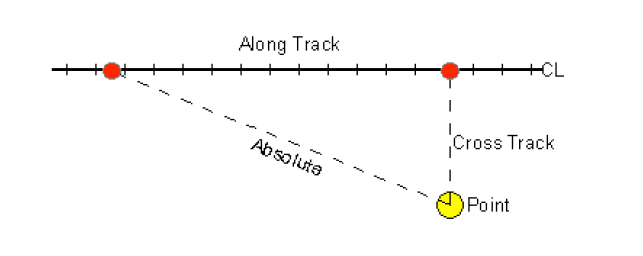
\includegraphics[width=3in]{graphics/AllenTrackRef.png}
			\caption{Track Centerline Accuracy Parameters~\citep{2006AllenAssetMap}}\label{fig:trackRef}
		\end{center}
	\vspace{-30pt}
\end{figure}
Other track asset mapping systems exist for determining the location and type of of assets held by railroads. The Union Pacific Railroad has developed and markets a HiRail-based measurement vehicle built on a SUV chassis and referred to as the Precision Measurement Vehicle (PMV). The PMV is used to provide location and description of all assets that can be measured from the railway. While occupying active mainline track, PMV operators use several measurement technologies to determine asset location. Four independent encoded wheels provide linear referenced track position inputs by by accumulating the slope distance between wayside monuments. A differential GPS receiver provides mapping-grade absolute position, while a fiber optic gyroscope (OG) is used to measure grade. The OG also serves to dampen the elevation observations from the DGPS reciever. A video interface provides the operator with a view through optical distance measuring instruments. A video recorder provides a record for milepost tracking and a survey log. Comparative positions generated by the PMV were not available for examination~\citep{2008pmv}.

Glaus details the development of a lightweight multi-sensor track surveying platform. The 99-pound (45 kg) hand-propelled device, nicknamed the \emph{Swiss Trolley}, tested several sensors and the development of a rigorous mathematical model for calculating kinematic track location. Close tolerance rail alinements are required for high speed passenger rail service. The \emph{Swiss Trolley} fills the need for precision track surveying by demonstrated the ability to determine absolute track axis\footnote{Referred to here as centerline top-of rail.} position to a high degree of precision. The \emph{Swiss Trolley} sensor suite is summarized in table \ref{tab:SwissTrolley}.

% Table of instruments: Glaus
\begin{table}[ht]
\begin{center}
	\caption{Swiss Trolley Instruments~\citep{2006glaus}}\label{tab:SwissTrolley}
	\begin{tabular}{ lll }
	\toprule
	Measurement & Sensor & Range/Resolution\\
	\midrule
	Absolute position & RTK GPS Total Station & 1 mm [sic]\\
	Absolute/relative position & Tracking Total Station & 1 mm\\
	Linear distance & Odometer & 0.08 mm\\
	Cross level/Grade & Inclinometer & $\pm$15$^{\circ}$\\
	Asset location & Laser scanner & 180$^{\circ}$\\
	& & 1 mm @ 32 m\\
	& & 10 mm @ 80 m\\
	Gauge & Angular transducer/rail contact & 0-45$^{\circ}$ \\
	\bottomrule
	\end{tabular}
\end{center}
\end{table}

Analog sensors on the \emph{Swiss Trolley} are linked to a control and data acquisition computer by means of an analog to digital multiplexor. Sensors are synchronized with 1 pps timing pulses generated by the GPS receiver. The sensor suite provides inputs to the model to calculate track axis, grade, cross level, and gauge. Points of concern are raised by the author in dealing with thermal and electrical noise on the analog-to-digital (ADC) converter inputs from a variety of sensors. Electromagnetic compatibility interaction between instruments was addressed by reducing the length and attention to the orientation of cables between sensors and ADCs. Two fluid-damped pendulum sensors provide cross-level and grade inputs. These inclinometers are subject to errors from nuisance vibrations, temperature, and collimation (axis alignment) error. Thermal instability errors were reduced by installing the sensors in an instrument oven to maintain a constant temperature regardless of ambient conditions. Grade and cross-level sensor vibration is modeled as a pendulum and applied to track position corrections. Significant is Glaus's method of integrating auxiliary instruments using Kalman filtering techniques to produce spatial accuracies in the range of several millimeters in a complex dynamic application.

The \emph{Swiss Trolley} is capable of producing exceptional track position accuracies, but the hand propelled sensor suit is limited to a maximum speed of 3.3 mph. Survey speeds are intentionally kept at a minimal to reduce sensor synchronization uncertainty for the platform. The reduced rate also aids in providing an accurate absolute time tag for kinematic data collection~\citep{2006glaus}. In its present form, the tight instrument integration and slow survey speed of the \emph{Swiss Trolley} make this approach impractical for track inspections across wide areas.

\section{Mainline Track Horizontal Alinement}Mainline railways are periodically inspected with specialized ``track geometry cars'' for compliance with FRA mandated track alinement criteria or to meet more stringent rail company specifications~\citep{49CFR213D}~\citep{2009bright}. Alinement data recorded by a track geometry car determines position by use of an odometer for track location within a linear reference system relative to wayside monuments. Wayside references commonly referred to as mile posts range from permanent cast concrete to steel signposts inserted into the ballast. Mile markers are subject to destruction or displacement from routine track maintenance and vandalism. Resetting mile posts is many times a best guess effort. Track geometry car measurements are typically referenced to these reference marks. Track defects referencing offsets from these marks are sometimes difficult to locate by Hi-Rail odometer.~\citep{2009vanPelt}.

The linear measurement system of a track geometry car produces accurate relative positions in the search to alinement defects. A geometry car will use GPS to provide a global reference frame to map alinement exceptions, however the accuracy of these GPS measurements are not adequate for use as a primary alinement tool. Track geometry vehicle inspections are limited in frequency due to the number of vehicles available, with those focused on higher traffic  segments.~\citep{2009bright.rtrack}.

\section{Track Occupancy}The FRA has established that any location determination system suitable for supporting positive train control must establish track occupancy with a very high degree of certainty. In a given parallel, multitrack segment, an LDS must be able to determine which track a given train is on without error. The FRA therefore requires a LDS to demonstrate track position that assumes a minimum track separation (center to center spacing) of 11.5 feet with 99.999\% confidence~\citep[4-5]{1995FRADiffe}.

A method of autonomous locomotive location referenced by US patent 6,641,090 and follow on 7,209,810 \emph{Locomotive Location System and Method} disclose an apparatus integrating inertial navigation, GPS, and a wheel mounted odometer as a method by which track occupancy can be determined by a train traveling proximal to a turnout. The patent claims teach that the method is able to determine track occupancy when a locomotive travels through a turnout by engaging a Kalman filter to process noisy inputs from accelerometers orthogonal to the direction of travel as the locomotive is diverted from the tangent track into a turnout. The output is compared with predefined track parameters by computing the location and corresponding estimated error states derived from the inertial navigation system until the estimated error state matches a pre-determined feature, indicating the track for that instance is not the track occupied by the locomotive. The method does not teach how to distinguish track occupancy between parallel trackways~\citep{2007lockheed}.

Improving the USDOD\footnote{United States Department of Defense} guarantee of  12.8 meter horizontal accuracy from the Global Positioning System Standard Positioning Service requires that positions calculated by a GPS receiver be augmented to correct for delays induced in the SV\footnote{Space vehicle} signal's travel through the ionosphere and troposphere and a variety of instrument errors~\citep{2001DoDGPSperf}. Correctors transmitted to and processed by a capable receiver are able to compensate for errors and improve the position determined at the receiver's antenna. Correctors are derived from the difference between the instantaneous position calculated at a stationary reference receiver antenna and the actual location of the stationary antenna. The reference receiver determines the signal error for each SV in view of the antenna. The position differential is the product of all ``signals in space'' errors induced in the signal, zeros the clock error between the reference and mobile reciever. SV signal errors accumulate from orbit irregularities (i.e.\ gravitational effects, solar wind, or outdated ephemerides); satellite and receiver clock errors; ionospheric and tropospheric delay; and other identifiable factors~\citep{2004leick}. The reference and mobile receivers must receive the same SV signals for correctors to have an effect on the mobile receiver position accuracy~\citep{2008USDoT_NDGPS}.

Current federal government augmentation systems, the Wide Area Augmentation Systems (WAAS) sponsored by the Federal Aviation Administration and the National Differential GPS (NDGPS) sponsored by the US Coast Guard, provide civilian users with mapping-grade\footnote{Defined here and generally accepted as 1 to 3 meter horizontal accuracy} position accuracy. The USDOT\footnote{United States Department of Transportation} was given presidential authority to develop and promote the use of civilian GPS augmentation systems. 

%USDOT authority for GPS in transportation applications
Presidential Decision Directive National Science and Technology Council (NSTC-6), designating USDOT to serve as the lead agency within the U.S. Government for all Federal civilian GPS matters. NSTC-6 commissioned the USDOT to:
\begin{quotation}
``Develop and implement U.S. Government augmentations to the basic GPS for transportation applications.
\begin{itemize}
\firmlist
	\item In cooperation with the Departments of Commerce, Defense and State, take the lead in promoting commercial applications of GPS technologies and the acceptance of GPS and U.S. Government augmentations as standards in domestic and international transportation systems.
	\item In cooperation with other departments and agencies, coordinate U.S. Government-provided GPS civil augmentation systems to minimize cost and duplication of effort~\citep{1996NSTC-6}.''
\end{itemize}
\end{quotation}

Federal government provided GPS\footnote{Non-GPS augmentation to GNSS systems is not provided by federal government systems} signal augmentation can be categorized by the augmenting signal transmitter location into 1) Space Based Augmentation Systems (SBAS) which use geosynchronous satellites to relay corrections from ground reference stations to the user, and 2) Ground Based Augmentation Systems (GBAS) which transmit corrections from ground reference stations directly to the user.

\subsection{Space-Based Augmentation Systems}
Government sponsored and privately funded SBAS are available to civilian and commercial users. The FAA\footnote{Federal Aviation Administration} sponsors WAAS\footnote{Wide Area Augmentation System} for aviation users and consists of an integrity reference monitoring network, processing facilities, geostationary satellites, and control facilities. The central data processing sites generate navigation messages for retransmission to users by geostationary satellites. The information is modulated on the GPS-like signal and broadcast to the users from geostationary satellites. WAAS corrections result in horizontal accuracies of 0.481 to 1.521 meters with 95\% confidence across the continental United States~\citep{WAAS09}.

WAAS is limited to broadcasting differential corrections for only GPS SVs. As with any SV signal, the reception of correctors broadcast from a geostationary SBAS satellite can be adversely affected by foliage, terrain, and building shadowing along the signal path from the SBAS SV to the user. The USDOT cites signal shadowing effects from a single geostationary point source as an objectionable characteristic for the use in railroad applications. The signal shadowing characteristic is a primary objection to the use of an SBAS as part of an LDS by the FRA~\citep{2008USDoT_NDGPS}.

Commercial SBAS subscription services enable horizontal accuracies to 6 cm @95\%and are used primarily in precision agriculture applications which, due to their use in open fields, are relatively unaffected by loss of the correction signal on the north side\footnote{SV orbits viewed from the ground, are not present in northern segments.} of tree lines or terrain, and under heavy foliage cover~\citep{2005fugro}.

\subsection{Ground-Based Augmentation Systems}  %NDGPS
The National Differential GPS (NDGPS) is a GBAS that uses terrestrial Low Frequency (LF) radio in the 285-325 kHz band for transmitting correctors to NDGPS capable receivers. A desirable aspect of long wavelength\footnote{$\lambda$=922 to 1052 m (3,025 to 3,451 ft)} LF radio is ground wave propagation. LF digital signals are favored by the USDOT for communicating correctors due to signal reception at distances up to 250 miles distant from a terrestrial reference station transmitter and LF.

The accuracy of NDGPS augmentation degrades at a rate of $\pm$~6.6 parts per million (ppm) distant from the reference receiver\footnote{At a distance of 250 miles, a user could expect an additional horizontal error of $\pm$8.7 feet ($6.6\cdot\frac{250\cdot5,280}{1,000,000}$)}~\citep{2000FRA_gps_ant}. A USDOT report recognizes other problems in addition to the low data rate of the NDGPS signal, in that the signal
\begin{quotation}
``...is further degraded by computational and other uncertainties in user equipment and the ability of user equipment to compensate for other error sources such as multi-path interference and propagation distortions''~\citep{2008USDoT_NDGPS}.
\end{quotation} 

With these considerations, the USDOT selected NDGPS as the GBAS for transportation applications. The USDOT promotes NDGPS as the augmentation system of choice for enabling positive train control location determination systems. The FRA qualifies its support for NDGPS use in PTC by understanding the need for ``other supplemental techniques'' to meet the high degree of confidence required of an LDS~\citep{1995FRADiffe}. The USDOT \emph{2008 NDGPS Assessment Final Report} states that ``NDGPS with its current level of accuracy has not proven adequate for safety-level track separation information~\citep{2008USDoT_NDGPS}.''

\section{Real Time Kinematic Technology}
Augmentation technologies such as Real Time Kinematic (RTK), provide the capability of centimeter-level GPS positioning in real time while the receiver is in motion. RTK technology was assessed in the USDOT Final Report on NDGPS as poorly suited for positive train control. The reports states that
\begin{quotation}``As railroads continue to deploy CBTC\footnote{Communications Based Train Control} and similar GPS-based train management and asset management systems, they must survey the railroad in GPS coordinates. Railroads cover too much territory to practically employ mobile survey-grade reference stations for these surveys~\citep[pp.12]{2008USDoT_NDGPS}.''\end{quotation}
Transmitting RTK correctors to mobile users was characterized as requiring
\begin{quotation}``\ldots their own wireless link between the reference station and the user receiver, which is typically limited to line-of-sight. If the user moves out of range (radio range or line of sight) of the reference station, the reference station must be re-positioned, and the user must again wait for the reference station to achieve ``lock'' with the GPS satellites required for high accuracy~\citep{2008USDoT_NDGPS}.''\end{quotation}
The USDOTs summary disclaims the use of RTK augmentation as ``not usable for general transportation applications''\citep[ES-7]{2008USDoT_NDGPS}.

This research disputes the 2008 USDOT assessment as failing to acknowledge the convergence of several technological factors enabling survey-grade absolute position measurement over wide areas. Demand for high quality positioning from satellite systems has lead to a growth in the availability of public and private alternatives to mapping-grade federal augmentation services. A number of state transportation and geodetic survey departments are building their own GPS/GNSS reference networks, providing survey-grade augmentation at no or nominal cost~\cite{ODOTvrs,MDOTvrs,NCvrs,KYCORS}. Unlike federal systems, state and private systems are not limited to providing augmentation for only GPS SVs. State government systems provide correctors for both US and Russian SVs, as well as future GNSSs like Galileo and Compass.

Private investment in networked reference systems provides a market opportunity to profit from the need for survey quality GNSS. Delivering real time correctors to a mobile receiver is enabled by the increased capacity to transmit data to users in the field by a number of means. Wireless data transmission comes at a reasonable price, with data transmission rates several orders of magnitude greater than NDGPS. Data rates are an important consideration in planning for the increase in corrector quantity due to new GPS signals\footnote{L2C and L5}, an increase in the number of modernized GLONASS SV launches, and future signals from Galileo and Compass.

CORS networked within in a geographic area deliver observations as real time inputs to a virtual reference station server (VRS), which provides the capability of continuously estimating the distortions of SV carrier phase observables and supply correctors to mobile receivers.  Mobile receivers are capable of applying VRS server transmitted correctors to instantaneously refine local observations to an accuracy of several centimeters. Mobile RTK users can expect to achieve position accuracies of 1-2 centimeters horizontal and 2-3 centimeters vertical across an entire regional VRS network with 95\% confidence.

\section{Literature Review Summary}

Recent negative reports by the USDOT regarding the use of Real Time Kinematic satellite navigation systems to determine track location indicate a gap exists between the use of US government sponsored GBAS and regional state government sponsored RTK systems. There also exists a gap between dedicated inspection systems such as track geometry cars; NDGPS augmented IMUs like Allen's Hi-Rail; and sophisticated, multi sensor arrays like the \emph{Swiss Trolley}. Review of intellectual property claims indicate addition work exists in industry that seeks to integrate federally provided augmentation with IMUs. It is unclear if intellectual property claims have been incorporated into commercial products to provide wireless locomotive location.

RTK infrastructure receivers networked to a VRS server combined with ubiquitous wireless data form a relatively new technology that enable absolute position measurement to within a centimeter over wide areas. It is the unexplored capability of RTK GNSS over the railway that establishes the need for this research in railroad transportation.

The research bridges a cap between mapping-grade track asset surveys that rely on mapping-grade US government provided GPS correctors, and complex track survey systems. This study examined the ability of RTK augmentation to bridge the gap to enable track measurement in applications not achievable through US government supplied augmentation services.
